\documentclass[table]{beamer}
\mode<presentation>
\usetheme{Berlin}
\usecolortheme{beaver}
\usepackage{listings}
\usepackage{multirow}

%%%
% TITLE PREAMBLE
\title[Intro to Bioinformatics] % (optional, only for long titles)
{An Introduction to Bioinformatics Tools}
\subtitle{Part 2: BLAST}
\author[Pritchard, Cock] % (optional, for multiple authors)
{Leighton~Pritchard \and Peter~Cock}
\institute[The James Hutton Institute] % (optional)
{
  Information and Computational Sciences\\
  The James Hutton Institute
}
\date[May 2014] % (optional)
{Bioinformatics Training, 29$^{th}$,30$^{th}$ May 2014}
\subject{Bioinformatics}

%%%
% TOC
% Show table of contents, with current section highlighted,
% at the start of each section
\AtBeginSection[]
{
  \begin{frame}
    \frametitle{Table of Contents}
    \tableofcontents[currentsection,hideothersubsections]
  \end{frame}
}


%%%
% START DOCUMENT
\begin{document}

  \frame[plain]{\titlepage}
  
%%%
% SECTION: BLAST Essentials
  \section{BLAST Essentials}
  
    % What is BLAST
    \subsection{What is BLAST?}
    \begin{frame}
     \frametitle{What BLAST Is}
     \begin{itemize}
       \item<1-> BLAST:
       \begin{itemize}
         \item<1-> Basic (it's actually sophisticated)
         \item<1-> Local Alignment (what it does: local sequence alignment)
         \item<1-> Search Tool (what it does: search against a database)
       \end{itemize}
       \item<2-> The most important software package in bioinformatics?
       \item<2-> Fast, robust, sequence similarity search tool
       \item<2-> Not foolproof.
     \end{itemize}
    \end{frame}
  
    \begin{frame}
     \frametitle{What A BLAST Search Is}
     \begin{itemize}
       \item BLAST search = identification of similar sequences in a database
       \item Results depend on:
       \begin{itemize}
         \item query sequence
         \item BLAST program (and choice of BLAST/BLAST+, version No.)
         \item database
         \item parameters
       \end{itemize}
     \end{itemize}
    \end{frame}  
  
    % Sequence Alignment
    \subsection{Sequence Alignment}
%    \begin{frame}
%     \frametitle{Assumptions}
%     You are familiar with
%     \begin{itemize}
%       \item biological sequences (RNA, DNA, protein)
%       \item mutation, drift, molecular clocks
%       \item gene and genome structure (including repeats, pseudogenes etc.)
%       \item homology, paralogy, orthology, etc.
%     \end{itemize}
%     - all important for interpretation of BLAST output
%    \end{frame}

    \begin{frame}
     \frametitle{Alignment Search Space}
     Consider two biological sequences to be aligned$\ldots$
     \begin{itemize}
       \item One sequence on the \textit{x}-axis, the other on the \textit{y}-axis
       \item Each point in space is a pairing of two letters
       \item Ungapped alignments are diagonal lines in the search space, gapped alignments have short 'breaks'
       \item There may be one or more "optimal" alignments
     \end{itemize}
     \begin{center}
       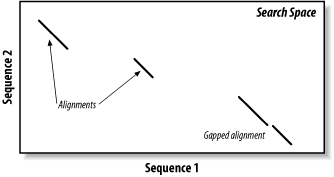
\includegraphics[width=0.4\textwidth]{images/search_space} 
     \end{center}
   \end{frame}
    
    \begin{frame}
     \frametitle{Global \textit{vs} Local Alignment}
     \begin{itemize}
       \item<1-> Global alignment: sequences are aligned along their entire lengths
       \item<1-> Local alignment: the best subsequence alignment is found
       \item<2-> Consider an alignment of the same gene from two distantly-related eukaryotes, where:
         \begin{itemize}
           \item<2-> Exons are conserved and small in relation to gene locus size
           \item<2-> Introns are not well-conserved but large in relation to gene locus size
         \end{itemize}
       \item<2-> Local alignment will align the conserved exon regions
       \item<2-> Global alignment will align the whole (mostly unrelated) locus
     \end{itemize}
    \end{frame}

    % dynamic programming
	\subsection{Dynamic Programming}
    \begin{frame}
     \frametitle{Our Goal}
     \begin{itemize}
       \item<1-> We aim to align the words
       \begin{itemize}
         \item<1-> \texttt{COELACANTH}
         \item<1-> \texttt{PELICAN}
       \end{itemize}
       \item<2-> Each identical letter (match) scores +1
       \item<2-> Each different letter (mismatch) scores -1
       \item<2-> Each gap scores -1
       \item<3-> \emph{Alignment is maximisation of the alignment score}
     \end{itemize}
    \end{frame}   
   
    \begin{frame}
     \frametitle{Initialise the matrix}
       \begin{center}
         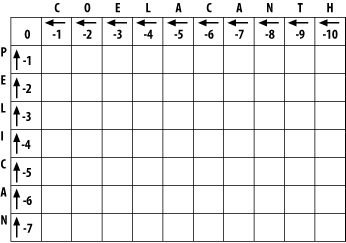
\includegraphics[width=0.5\textwidth]{images/initialise}
       \end{center}
    \end{frame}   
   
    \begin{frame}
     \frametitle{Fill the cells}
       \begin{center}
         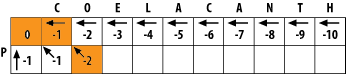
\includegraphics[width=0.5\textwidth]{images/fill_start} \\
         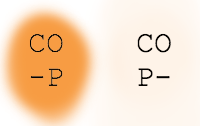
\includegraphics[width=0.3\textwidth]{images/fill_start_letters}
       \end{center}
    \end{frame}     

    \begin{frame}
     \frametitle{Fill the matrix}
       \begin{center}
         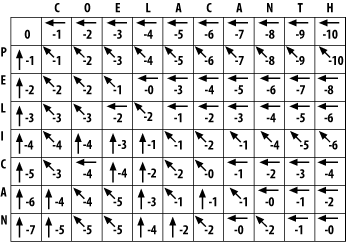
\includegraphics[width=0.5\textwidth]{images/full_matrix}
       \end{center}
       Matrix represents all possible pairwise alignments and scores
    \end{frame}  
   
    \begin{frame}
     \frametitle{Traceback}
       \begin{center}
         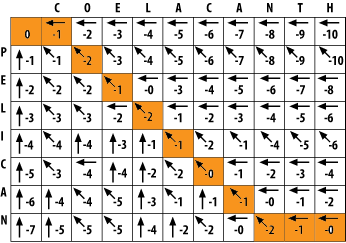
\includegraphics[width=0.5\textwidth]{images/traceback} \\
         
\includegraphics[width=0.3\textwidth]{images/traceback_sequence}         
       \end{center}
    \end{frame}     

    \begin{frame}
     \frametitle{Algorithms}
       \begin{itemize}
         \item<1-> Global: Needleman-Wunsch (as in example)
         \item<1-> Local: Smith-Waterman (differs from example)
         \item<2-> NW/SW are \emph{guaranteed} to find the optimal match \emph{with respect to the scoring system being used}
         \item<2-> Alignment is an approximation: no scoring scheme encapsulates biological "truth"
         \item<2-> Any pair of sequences can be aligned: finding meaning is up to you
       \end{itemize}
    \end{frame}   

%    \begin{frame}
%     \frametitle{Dynamic Programming}
%     \framesubtitle{Gap Scoring}
%       \begin{itemize}
%         \item Simple gap penalty: all gaps score the same
%         \begin{itemize}
%           \item \emph{one} parameter in the alignment model
%         \end{itemize}
%         \item Affine gap penalty: opening and extending score differently
%         \begin{itemize}
%           \item \emph{two} parameters in the alignment model
%         \end{itemize}
%       \end{itemize}
%       \begin{center}
%         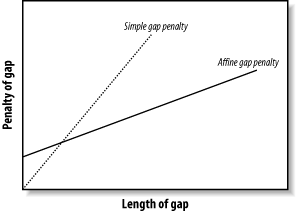
\includegraphics[width=0.3\textwidth]{images/gap_scores} 
%       \end{center}
%     \end{frame}  
   
%    \begin{frame}
%     \frametitle{Dynamic Programming}
%     \framesubtitle{Banded Alignment}
%       \begin{itemize}
%         \item Given a maximum scoring alignment, restrict search to a "band" between endpoints
%         \item Width of this band = "bandwidth", another parameter in the model (may be floating)
%         \item Speeds up search, reduces memory use
%       \end{itemize}
%       \begin{center}
%         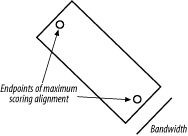
\includegraphics[width=0.3\textwidth]{images/banded} 
%       \end{center}
%     \end{frame}     


    % The BLAST Algorithm
    \section{The BLAST Algorithm}
    \begin{frame}
     \frametitle{BLAST Is A Heuristic}
     \begin{itemize}
       \item<1-> BLAST does not use Needleman-Wunsch or Smith-Waterman
       \item<1-> BLAST \emph{approximates} dynamic programming methods
       \item<1-> BLAST is not guaranteed to give an optimal alignment (for chosen parameters)
       \item<2-> BLAST does not explore the complete search space
       \item<3-> BLAST uses heuristics (loosely-defined rules) to refine High-scoring Segment Pairs (HSPs)
       \item<4-> BLAST reports only "statistically-significant" alignments (dependent on parameters)
     \end{itemize}
   \end{frame}

  \begin{frame}
    \frametitle{Steps in the Algorithm}
    \begin{enumerate}
      \item Seeding
      \item Extension
      \item Evaluation
    \end{enumerate}
  \end{frame}

%  \begin{frame}
%    \frametitle{About BLAST databases$\ldots$}
%    \begin{itemize}
%      \item The database used is a parameter in your model
%      \item Three components:
%      \begin{itemize}
%        \item header file: \texttt{*.phr}, \texttt{*.nhr}
%        \item sequence file: \texttt{*.psq}, \texttt{*.nsq}
%        \item index file: \texttt{*.pin}, \texttt{*.nin}
%      \end{itemize}
%      \item The index allows for fast searching                
%    \end{itemize}
%  \end{frame}

  % seeding
  \subsection{Seeding}
  \begin{frame}
    \frametitle{Word Hit}
    \begin{itemize}
      \item A short sequence and its \emph{neighbourhood}
      \item \emph{neighbourhood}: words of same length whose aligned score is greater than or equal to a threshold value $T$
      \item Three parameters: scoring matrix, word size $W$, and $T$
    \end{itemize}
    \begin{center}
      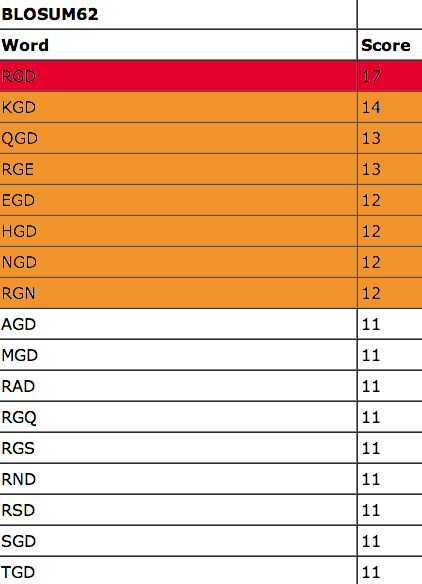
\includegraphics[width=0.3\textwidth]{images/neighbourhood} 
    \end{center}    
  \end{frame}

  \begin{frame}
    \frametitle{Seeding}
    \begin{itemize}
      \item BLAST assumption: significant alignments have \emph{words} in common
      \item BLAST finds word (\emph{neighbourhood}) hits in the database index
      \item Word hits are used to \textit{seed} alignments
    \end{itemize}
    \begin{center}
      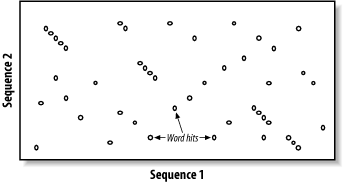
\includegraphics[width=0.5\textwidth]{images/seeding} 
    \end{center}    
  \end{frame}

  \begin{frame}
    \frametitle{Seeding Controls Sensitivity}
    \begin{itemize}
      \item Word size $W$ controls number of hits (smaller words $\implies$ more hits)
      \item Threshold score $T$ controls number of hits (lower threshold $\implies$ more hits)
      \item Scoring matrix controls which words match
    \end{itemize}
    \begin{center}
      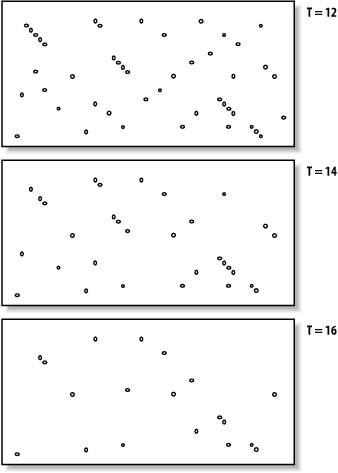
\includegraphics[width=0.25\textwidth]{images/seeding_t} 
    \end{center}    
  \end{frame}

  \begin{frame}
    \frametitle{The Two-Hit Algorithm}
    \begin{itemize}
      \item BLAST assumption: word hits cluster on the diagonal for significant alignments
      \item The acceptable distance $A$ between words on the diagonal is a parameter of your model
      \item Smaller distances isolate single words, and reduce search space
    \end{itemize}
    \begin{center}
      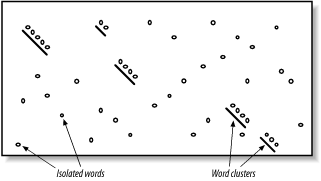
\includegraphics[width=0.5\textwidth]{images/two_hit} 
    \end{center}    
  \end{frame}

  % extension
  \subsection{Extension}
  \begin{frame}
    \frametitle{Extension}
    \begin{itemize}
      \item The best-scoring seeds are extended in each direction
      \item BLAST does not explore the complete search space, so a rule (heuristic) to stop extension is needed
      \item Two-stage process:
      \begin{itemize}
        \item Extend, keeping alignment score, and \emph{drop-off} score
        \item When drop-of score reaches a threshold $X$, trim alignment back to top score
      \end{itemize}
    \end{itemize}
    \begin{center}
      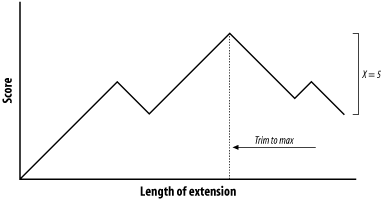
\includegraphics[width=0.5\textwidth]{images/extension} 
    \end{center}    
  \end{frame}

  \begin{frame}
    \frametitle{Example}
    \begin{itemize}
      \item<1-> Consider two sentences (match=+1, mismatch=-1)
      \begin{itemize}
        \item \texttt{The quick brown fox jumps over the lazy dog.}
        \item \texttt{The quiet brown cat purrs when she sees him.}
      \end{itemize}
      \item<2-> Extend to the right from the seed \texttt{T}
      \begin{itemize}
        \item \texttt{The quic}
        \item \texttt{The quie}
        \item \texttt{123 4565 <- score}
        \item \texttt{000 0001 <- drop-off score}        
      \end{itemize}
    \end{itemize}
  \end{frame}

  \begin{frame}
    \frametitle{Example}
    \begin{itemize}
      \item Consider two sentences (match=+1, mismatch=-1)
      \begin{itemize}
        \item \texttt{The quick brown fox jumps over the lazy dog.}
        \item \texttt{The quiet brown cat purrs when she sees him.}
      \end{itemize}
      \item Extend to drop-off threshold
      \begin{itemize}
        \item \texttt{The quick brown fox jump}
        \item \texttt{The quiet brown cat purr}
        \item \texttt{123 45654 56789 876 5654 <- score}
        \item \texttt{000 00012 10000 123 4345 <- drop-off score}        
      \end{itemize}
    \end{itemize}
  \end{frame}

  \begin{frame}
    \frametitle{Example}
    \begin{itemize}
      \item Consider two sentences (match=+1, mismatch=-1)
      \begin{itemize}
        \item \texttt{The quick brown fox jumps over the lazy dog.}
        \item \texttt{The quiet brown cat purrs when she sees him.}
      \end{itemize}
      \item Trim back from drop-off threshold to get optimal alignment
      \begin{itemize}
        \item \texttt{The quick brown}
        \item \texttt{The quiet brown}
        \item \texttt{123 45654 56789 <- score}
        \item \texttt{000 00012 10000 <- drop-off score}        
      \end{itemize}
    \end{itemize}
  \end{frame}

  \begin{frame}
    \frametitle{Notes on implementation}
    \begin{itemize}
%      \item This example represents ungapped BLAST; gapped BLAST is more similar to dynamic programming
      \item $X$ controls termination of alignment extension, but dependent on:
      \begin{itemize}
        \item substitution matrix
        \item gap opening and extension parameters
      \end{itemize}
    \end{itemize}
    \begin{center}
      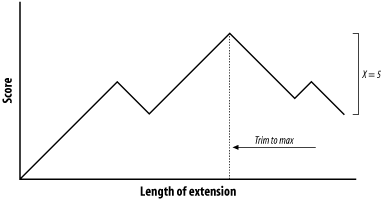
\includegraphics[width=0.5\textwidth]{images/extension} 
    \end{center}    
  \end{frame}

  % evaluation
  \subsection{Evaluation}
  \begin{frame}
    \frametitle{Evaluation}
    \begin{itemize}
      \item The principle is easy: use a score threshold $S$ to determine strong and weak alignments
      \begin{itemize}
        \item $S$ is monotonic with $E$, so an equivalent threshold can be calculated
      \end{itemize}
      \item Score $S$ is independent of database size and search space. $E$ values are not.
      \item Alignment consistency is also a consideration
    \end{itemize}
    \begin{center}
      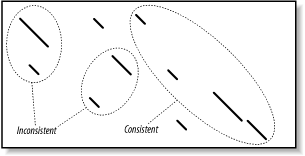
\includegraphics[width=0.5\textwidth]{images/consistency} 
    \end{center}    
  \end{frame}


  % BLAST statistics
  \section{BLAST Statistics}
  
%    % Information Theory
%    \subsection{Information Theory}
%    \begin{frame}
%     \frametitle{Bits of Information}
%     \begin{itemize}
%       \item<1-> The amount of information in a thing (e.g. a message, or picture) can be measured in \emph{bits}, and represented as $H$ (entropy)
%       \item<1-> One bit = one "yes/no" or "1/0" answer
%       \item<2-> The information associated with a probability $p$ can be represented in bits: \\
%                 $H(p) = -\text{log}_2(p)$
%       \item<2-> For a series of $n$ probabilities $\{p_i,$\ldots$, p_n\}$ we have: \\
%                 $H = -\sum^{n}_{i} p_i \text{log}_2 (p_i)$
%     \end{itemize}
%    \end{frame}
%
%    \begin{frame}
%     \frametitle{Information in Random Alphabets}
%     \begin{itemize}
%       \item DNA and protein alphabets have multiple symbols, so have different entropies (are not equally informative)
%       \item Assuming random sequences (no symbol bias):
%       \begin{itemize}
%         \item For a coin, $p(H) = p(T) = 0.5 \implies H(coin) = 1\text{bit}$
%         \item For DNA, $p(A) = p(C) = p(G) = p(T) = 0.25 \implies H(\text{DNA}) = 2\text{bits}$       
%         \item For protein, $p(A) = p(C) = $\ldots$ = 0.05 \implies H(\text{protein}) = 4.32\text{bits}$
%       \end{itemize}
%       \item Twice as much information in protein than DNA alphabet
%     \end{itemize}
%    \end{frame}
%
%    \begin{frame}
%     \frametitle{Information in Biased Alphabets}
%     \begin{itemize}
%       \item Deviation from random sequence reduces entropy
%       \begin{itemize}
%         \item For DNA, $p(A) = p(C) = p(G) = p(T) = 0.25 \implies H(\text{DNA}) = 2\text{bits}$       
%         \item For DNA: $p(A) = 0.4; p(C) = 0.3; p(G) = 0.2; p(T) = 0.1 \implies H(\text{DNA}) = 1.85\text{bits}$       
%       \end{itemize}
%       \item Biological sequences/databases deviate from randomness
%     \end{itemize}
%    \end{frame}
%  
    % Substitution matrices
    \subsection{Substitution Matrices}
%    \begin{frame}
%     \frametitle{Log-odds Scores}
%     \begin{itemize}
%       \item<1-> How often does a symbol substitution occur, compared to random expectation?
%       \item<1-> If $p(\text{Met}) = 0.01$, $p(\text{Leu}) = 0.1$, we would expect a Met-Leu substitution with frequency $p(\text{Met})p(\text{Leu}) = 0.001$
%       \item<2-> Observe Met-Leu substitution with frequency $q(\text{Met-Leu}) = 0.002$
%       \item<2-> Odds ratio is $\frac{q(\text{Met-Leu})}{p(\text{Met})p(\text{Leu})} = 2$
%       \item<3-> Log odds ratio is $\text{log}_2(\frac{q(\text{Met-Leu})}{p(\text{Met})p(\text{Leu})}) = 1\text{bit}$
%     \end{itemize}
%    \end{frame}  

    \begin{frame}
     \frametitle{Log-odds Matrices}
     \begin{itemize}
       \item Substitution matrices are a model of evolution, represented by log-odds matrices
       \begin{itemize}
         \item Positive numbers indicate likely substitutions/similarity
         \item Negative numbers indicate unlikely substitutions/dissimilarity
       \end{itemize}
     \end{itemize}
    \begin{center}
      BLOSUM62 \\
      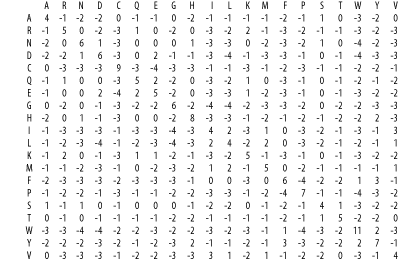
\includegraphics[width=0.5\textwidth]{images/blosum62} 
    \end{center}         
    \end{frame} 

    \begin{frame}
     \frametitle{Choice of Matrix}
     \begin{itemize}
       \item Substitution matrix determines the raw alignment score $S$
       \begin{itemize}
         \item $S$ is the sum of pairwise scores in an alignment
       \end{itemize}
       \item For proteins:
       \begin{itemize}
         \item \texttt{BLOSUM45 BLOSUM50 BLOSUM62 BLOSUM80 BLOSUM90}
         \item \texttt{PAM30 PAM70 PAM250}
       \end{itemize}
       \item BLOSUM matrices empirically defined from multiple sequence alignments of $\geq n\%$ identity, for \texttt{BLOSUMn}
       \item For nucleotides: 'matrix' defined by match/mismatch (reward/penalty) parameters
     \end{itemize}
    \end{frame} 
  
%    \begin{frame}
%     \frametitle{Target Frequencies}
%     \begin{itemize}
%       \item Target frequencies represent the underlying evolutionary model implicit in the substitution matrix
%       \item Each substitution matrix has a scaling factor $\lambda$, estimated from symbol frequency
%       \item $\lambda$ is used to calculate a \emph{normalised score} for the alignment, $\lambda S$
%       \item In modern BLAST, $\lambda$ is also dependent on the query and subject sequence composition
%     \end{itemize}
%    \end{frame}   

%    \begin{frame}
%     \frametitle{Substitution Matrices}
%     \framesubtitle{matrix relative entropy}
%     \begin{itemize}
%       \item Matrix \emph{expected score} $E$ is the sum of raw scores weighted by frequency of occurrence (should be negative)
%       \begin{equation}
%         E = \sum^{20}_{i=1}\sum_{j=1}^{i} p_i p_j S_{ij}
%       \end{equation}
%       \item Matrix \emph{relative entropy} $H$ is the average number of bits per position in an alignment generated from that matrix.
%       \begin{equation}
%         H = \sum^{20}_{i=1}\sum_{j=1}^{i} q_{ij} \lambda S_{ij}
%       \end{equation}
%     \end{itemize}
%    \end{frame} 

    % Karlin-Altschul Equation
    \subsection{Karlin-Altschul Equation}
    \begin{frame}
     \frametitle{Definition}
     \begin{itemize}
       \item The Karlin-Altschul equation
       \begin{equation*}
         E = k m n e^{-\lambda S}
       \end{equation*}
       \item Symbols:
       \begin{itemize}
         \item $k$: minor constant, adjusts for correlation between alignments
         \item $m$: number of letters in query sequence
         \item $n$: number of letters in the database
         \item $\lambda$: scoring matrix scaling factor
         \item $S$: raw alignment score
       \end{itemize}
     \end{itemize}
    \end{frame} 

%    \begin{frame}
%     \frametitle{Assumptions}
%     \begin{itemize}
%       \item The Karlin-Altschul equation
%       \begin{equation*}
%         E = k m n e^{-\lambda S}
%       \end{equation*}
%       \item Assumptions:
%       \begin{itemize}
%         \item A positive score must be possible
%         \item The scoring matrix \emph{expected score} must be negative
%         \item Sequences are infinitely long
%         \item Alignments do not contain gaps
%         \item Sequence symbols (bases, residues) are independent and identically-distributed
%       \end{itemize}
%     \end{itemize}
%    \end{frame} 

    \begin{frame}
     \frametitle{Interpretation}
     \begin{itemize}
       \item The Karlin-Altschul equation
       \begin{equation*}
         E = k m n e^{-\lambda S}
       \end{equation*}
       \item $E$ is the number of alignments with a similar score expected by chance when querying a database of that size and symbol frequency, where the letters in the database are randomly-ordered
       \item Small changes in score $S$ can produce large changes in $E$
       \item Biological sequence databases are not random!
     \end{itemize}
    \end{frame} 

  
  % Using BLAST   
  \section{Using BLAST}
    \subsection{Which BLAST tool should I use?}
    \begin{frame}
     \frametitle{}
    \end{frame}

    \subsection{Controlling BLAST output}
    \begin{frame}
     \frametitle{}
    \end{frame}
     
    \subsection{Interpreting BLAST output}
    \begin{frame}
     \frametitle{}
    \end{frame}
    
% etc
\end{document}